\documentclass[letterpaper,12pt,twoside,]{pinp}

%% Some pieces required from the pandoc template
\providecommand{\tightlist}{%
  \setlength{\itemsep}{0pt}\setlength{\parskip}{0pt}}

% Use the lineno option to display guide line numbers if required.
% Note that the use of elements such as single-column equations
% may affect the guide line number alignment.

\usepackage[T1]{fontenc}
\usepackage[utf8]{inputenc}

% pinp change: the geometry package layout settings need to be set here, not in pinp.cls
\geometry{layoutsize={0.95588\paperwidth,0.98864\paperheight},%
  layouthoffset=0.02206\paperwidth, layoutvoffset=0.00568\paperheight}

\definecolor{pinpblue}{HTML}{185FAF}  % imagecolorpicker on blue for new R logo
\definecolor{pnasbluetext}{RGB}{101,0,0} %



\title{Lab 004 - Normal curve calculations - Solutions.}

\author[a]{EPIB607 - Inferential Statistics}

  \affil[a]{Fall 2020, McGill University}

\setcounter{secnumdepth}{5}

% Please give the surname of the lead author for the running footer
\leadauthor{Bhatnagar}

% Keywords are not mandatory, but authors are strongly encouraged to provide them. If provided, please include two to five keywords, separated by the pipe symbol, e.g:
 \keywords{  Sampling distribution |  Standard error |  Normal distribution |  Quantiles |  Percentiles |  Z-scores  }  

\begin{abstract}
Because the results of random samples include an element of chance, we
can't guarantee that our inferences are correct. What we can guarantee
is that our methods usually give correct answers. We will see that the
reasoning of statistical inference rests on asking ``How often would
this method give a correct answer if I used it very many times ?'' To be
able to answer these questions we need to understand sampling
distributions and the normal curve. In this exercise you will practice
calculating quantiles and probablities from the Normal distribution.
\end{abstract}

\dates{This version was compiled on \today} 

% initially we use doi so keep for backwards compatibility
% new name is doi_footer

\pinpfootercontents{in-class exercise on pnorm qnorm}

\begin{document}

% Optional adjustment to line up main text (after abstract) of first page with line numbers, when using both lineno and twocolumn options.
% You should only change this length when you've finalised the article contents.
\verticaladjustment{-2pt}

\maketitle
\thispagestyle{firststyle}
\ifthenelse{\boolean{shortarticle}}{\ifthenelse{\boolean{singlecolumn}}{\abscontentformatted}{\abscontent}}{}

% If your first paragraph (i.e. with the \dropcap) contains a list environment (quote, quotation, theorem, definition, enumerate, itemize...), the line after the list may have some extra indentation. If this is the case, add \parshape=0 to the end of the list environment.


\hypertarget{normal-probability-calculations}{%
\section{Normal probability
calculations}\label{normal-probability-calculations}}

Using your method of choice, calculate the following probabilities
assuming \(Y\) is a standard normal distribution
(\(Y \sim \mathcal{N}(0,1)\)):

\begin{enumerate}
\def\labelenumi{\alph{enumi})}
\tightlist
\item
  \(P(Y < -1.80)\)
\item
  \(P(Y > -1.80)\)
\item
  \(P(Y \geq 1.60)\)
\item
  \(P(-1.8 < Y \leq 1.6)\)
\end{enumerate}

\begin{Shaded}
\begin{Highlighting}[]
\CommentTok{# default is always mean = 0, sd = 1, lower.tail=TRUE}
\CommentTok{# a)}
\NormalTok{mosaic}\OperatorTok{::}\KeywordTok{xpnorm}\NormalTok{(}\DataTypeTok{q =} \FloatTok{-1.80}\NormalTok{)}
\end{Highlighting}
\end{Shaded}

\begin{ShadedResult}
\begin{verbatim}
#  Registered S3 method overwritten by 'mosaic':
#    method                           from   
#    fortify.SpatialPolygonsDataFrame ggplot2
\end{verbatim}
\end{ShadedResult}
\begin{ShadedResult}
\begin{verbatim}
#  
\end{verbatim}
\end{ShadedResult}
\begin{ShadedResult}
\begin{verbatim}
#  If X ~ N(0, 1), then
\end{verbatim}
\end{ShadedResult}
\begin{ShadedResult}
\begin{verbatim}
#   P(X <= -1.8) = P(Z <= -1.8) = 0.03593
\end{verbatim}
\end{ShadedResult}
\begin{ShadedResult}
\begin{verbatim}
#   P(X >  -1.8) = P(Z >  -1.8) = 0.9641
\end{verbatim}
\end{ShadedResult}
\begin{ShadedResult}
\begin{verbatim}
#  
\end{verbatim}
\end{ShadedResult}

\begin{center}
\includegraphics{004-pnorm-qnorm-exercise-solutions_files/figure-latex/unnamed-chunk-1-1} \end{center}

\begin{ShadedResult}
\begin{verbatim}
#  [1] 0.03593032
\end{verbatim}
\end{ShadedResult}

\begin{Shaded}
\begin{Highlighting}[]
\CommentTok{# b)}
\NormalTok{mosaic}\OperatorTok{::}\KeywordTok{xpnorm}\NormalTok{(}\DataTypeTok{q =} \FloatTok{-1.80}\NormalTok{, }\DataTypeTok{lower.tail =} \OtherTok{FALSE}\NormalTok{)}
\end{Highlighting}
\end{Shaded}

\begin{ShadedResult}
\begin{verbatim}
#  
\end{verbatim}
\end{ShadedResult}
\begin{ShadedResult}
\begin{verbatim}
#  If X ~ N(0, 1), then
\end{verbatim}
\end{ShadedResult}
\begin{ShadedResult}
\begin{verbatim}
#   P(X <= -1.8) = P(Z <= -1.8) = 0.03593
\end{verbatim}
\end{ShadedResult}
\begin{ShadedResult}
\begin{verbatim}
#   P(X >  -1.8) = P(Z >  -1.8) = 0.9641
\end{verbatim}
\end{ShadedResult}
\begin{ShadedResult}
\begin{verbatim}
#  
\end{verbatim}
\end{ShadedResult}

\begin{center}
\includegraphics{004-pnorm-qnorm-exercise-solutions_files/figure-latex/unnamed-chunk-1-2} \end{center}

\begin{ShadedResult}
\begin{verbatim}
#  [1] 0.9640697
\end{verbatim}
\end{ShadedResult}

\begin{Shaded}
\begin{Highlighting}[]
\CommentTok{# c)}
\NormalTok{mosaic}\OperatorTok{::}\KeywordTok{xpnorm}\NormalTok{(}\DataTypeTok{q =} \FloatTok{1.60}\NormalTok{, }\DataTypeTok{lower.tail =} \OtherTok{FALSE}\NormalTok{)}
\end{Highlighting}
\end{Shaded}

\begin{ShadedResult}
\begin{verbatim}
#  
\end{verbatim}
\end{ShadedResult}
\begin{ShadedResult}
\begin{verbatim}
#  If X ~ N(0, 1), then
\end{verbatim}
\end{ShadedResult}
\begin{ShadedResult}
\begin{verbatim}
#   P(X <= 1.6) = P(Z <= 1.6) = 0.9452
\end{verbatim}
\end{ShadedResult}
\begin{ShadedResult}
\begin{verbatim}
#   P(X >  1.6) = P(Z >  1.6) = 0.0548
\end{verbatim}
\end{ShadedResult}
\begin{ShadedResult}
\begin{verbatim}
#  
\end{verbatim}
\end{ShadedResult}

\begin{center}
\includegraphics{004-pnorm-qnorm-exercise-solutions_files/figure-latex/unnamed-chunk-1-3} \end{center}

\begin{ShadedResult}
\begin{verbatim}
#  [1] 0.05479929
\end{verbatim}
\end{ShadedResult}

\begin{Shaded}
\begin{Highlighting}[]
\CommentTok{# d)}
\KeywordTok{pnorm}\NormalTok{(}\DataTypeTok{q =} \FloatTok{1.60}\NormalTok{) }\OperatorTok{-}\StringTok{ }\KeywordTok{pnorm}\NormalTok{(}\DataTypeTok{q =} \FloatTok{-1.80}\NormalTok{)}
\end{Highlighting}
\end{Shaded}

\begin{ShadedResult}
\begin{verbatim}
#  [1] 0.9092704
\end{verbatim}
\end{ShadedResult}

\begin{Shaded}
\begin{Highlighting}[]
\NormalTok{mosaic}\OperatorTok{::}\KeywordTok{xpnorm}\NormalTok{(}\DataTypeTok{q =} \KeywordTok{c}\NormalTok{(}\OperatorTok{-}\FloatTok{1.80}\NormalTok{, }\FloatTok{1.60}\NormalTok{))}
\end{Highlighting}
\end{Shaded}

\begin{ShadedResult}
\begin{verbatim}
#  
\end{verbatim}
\end{ShadedResult}
\begin{ShadedResult}
\begin{verbatim}
#  If X ~ N(0, 1), then
\end{verbatim}
\end{ShadedResult}
\begin{ShadedResult}
\begin{verbatim}
#   P(X <= -1.8) = P(Z <= -1.8) = 0.03593   P(X <=  1.6) = P(Z <=  1.6) = 0.94520
\end{verbatim}
\end{ShadedResult}
\begin{ShadedResult}
\begin{verbatim}
#   P(X >  -1.8) = P(Z >  -1.8) = 0.9641    P(X >   1.6) = P(Z >   1.6) = 0.0548
\end{verbatim}
\end{ShadedResult}
\begin{ShadedResult}
\begin{verbatim}
#  
\end{verbatim}
\end{ShadedResult}

\begin{center}
\includegraphics{004-pnorm-qnorm-exercise-solutions_files/figure-latex/unnamed-chunk-1-4} \end{center}

\begin{ShadedResult}
\begin{verbatim}
#  [1] 0.03593032 0.94520071
\end{verbatim}
\end{ShadedResult}

\hypertarget{hdl-cholesterol}{%
\section{HDL cholesterol}\label{hdl-cholesterol}}

\begin{enumerate}
\def\labelenumi{\alph{enumi}.}
\tightlist
\item
  US women over the age of 19 have a mean (HDL) cholesterol measure of
  55 mg/dL with a standard deviation of 15.5 mg/dL. Assume HDL follows a
  Normal distribution.

  \begin{enumerate}
  \def\labelenumii{\roman{enumii}.}
  \tightlist
  \item
    What percent of women have low values of HDL, where low is defined
    to be 40 mg/dL or less?
  \item
    HDL levels of 60 mg/dL or more are believed to be protective against
    heart disease. What percent of women have protective levels of HDL?
  \item
    What proportion of women has HDL in the range of 40-60 mg/dL?
  \item
    What proportion of women has HDL in the range of 35-65 mg/dL?
  \end{enumerate}
\end{enumerate}

\begin{Shaded}
\begin{Highlighting}[]
\CommentTok{# i. }
\NormalTok{mosaic}\OperatorTok{::}\KeywordTok{xpnorm}\NormalTok{(}\DataTypeTok{q =} \DecValTok{40}\NormalTok{, }\DataTypeTok{mean =} \DecValTok{55}\NormalTok{, }\DataTypeTok{sd =} \FloatTok{15.5}\NormalTok{)}
\end{Highlighting}
\end{Shaded}

\begin{ShadedResult}
\begin{verbatim}
#  
\end{verbatim}
\end{ShadedResult}
\begin{ShadedResult}
\begin{verbatim}
#  If X ~ N(55, 15.5), then
\end{verbatim}
\end{ShadedResult}
\begin{ShadedResult}
\begin{verbatim}
#   P(X <= 40) = P(Z <= -0.9677) = 0.1666
\end{verbatim}
\end{ShadedResult}
\begin{ShadedResult}
\begin{verbatim}
#   P(X >  40) = P(Z >  -0.9677) = 0.8334
\end{verbatim}
\end{ShadedResult}
\begin{ShadedResult}
\begin{verbatim}
#  
\end{verbatim}
\end{ShadedResult}

\begin{center}
\includegraphics{004-pnorm-qnorm-exercise-solutions_files/figure-latex/unnamed-chunk-2-1} \end{center}

\begin{ShadedResult}
\begin{verbatim}
#  [1] 0.1665866
\end{verbatim}
\end{ShadedResult}

\begin{Shaded}
\begin{Highlighting}[]
\CommentTok{# ii. }
\NormalTok{mosaic}\OperatorTok{::}\KeywordTok{xpnorm}\NormalTok{(}\DataTypeTok{q =} \DecValTok{60}\NormalTok{, }\DataTypeTok{mean =} \DecValTok{55}\NormalTok{, }\DataTypeTok{sd =} \FloatTok{15.5}\NormalTok{, }\DataTypeTok{lower.tail =} \OtherTok{FALSE}\NormalTok{)}
\end{Highlighting}
\end{Shaded}

\begin{ShadedResult}
\begin{verbatim}
#  
\end{verbatim}
\end{ShadedResult}
\begin{ShadedResult}
\begin{verbatim}
#  If X ~ N(55, 15.5), then
\end{verbatim}
\end{ShadedResult}
\begin{ShadedResult}
\begin{verbatim}
#   P(X <= 60) = P(Z <= 0.3226) = 0.6265
\end{verbatim}
\end{ShadedResult}
\begin{ShadedResult}
\begin{verbatim}
#   P(X >  60) = P(Z >  0.3226) = 0.3735
\end{verbatim}
\end{ShadedResult}
\begin{ShadedResult}
\begin{verbatim}
#  
\end{verbatim}
\end{ShadedResult}

\begin{center}
\includegraphics{004-pnorm-qnorm-exercise-solutions_files/figure-latex/unnamed-chunk-2-2} \end{center}

\begin{ShadedResult}
\begin{verbatim}
#  [1] 0.3735064
\end{verbatim}
\end{ShadedResult}

\begin{Shaded}
\begin{Highlighting}[]
\CommentTok{# iii. }
\NormalTok{mosaic}\OperatorTok{::}\KeywordTok{xpnorm}\NormalTok{(}\DataTypeTok{q =} \KeywordTok{c}\NormalTok{(}\DecValTok{40}\NormalTok{,}\DecValTok{60}\NormalTok{), }\DataTypeTok{mean =} \DecValTok{55}\NormalTok{, }\DataTypeTok{sd =} \FloatTok{15.5}\NormalTok{)}
\end{Highlighting}
\end{Shaded}

\begin{ShadedResult}
\begin{verbatim}
#  
\end{verbatim}
\end{ShadedResult}
\begin{ShadedResult}
\begin{verbatim}
#  If X ~ N(55, 15.5), then
\end{verbatim}
\end{ShadedResult}
\begin{ShadedResult}
\begin{verbatim}
#   P(X <= 40) = P(Z <= -0.9677) = 0.1666   P(X <= 60) = P(Z <=  0.3226) = 0.6265
\end{verbatim}
\end{ShadedResult}
\begin{ShadedResult}
\begin{verbatim}
#   P(X >  40) = P(Z >  -0.9677) = 0.8334   P(X >  60) = P(Z >   0.3226) = 0.3735
\end{verbatim}
\end{ShadedResult}
\begin{ShadedResult}
\begin{verbatim}
#  
\end{verbatim}
\end{ShadedResult}

\begin{center}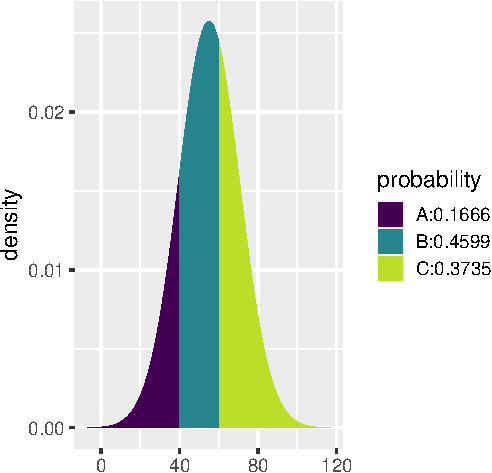
\includegraphics{004-pnorm-qnorm-exercise-solutions_files/figure-latex/unnamed-chunk-2-3} \end{center}

\begin{ShadedResult}
\begin{verbatim}
#  [1] 0.1665866 0.6264936
\end{verbatim}
\end{ShadedResult}

\begin{Shaded}
\begin{Highlighting}[]
\KeywordTok{pnorm}\NormalTok{(}\DataTypeTok{q =} \DecValTok{60}\NormalTok{, }\DataTypeTok{mean =} \DecValTok{55}\NormalTok{, }\DataTypeTok{sd =} \FloatTok{15.5}\NormalTok{) }\OperatorTok{-}\StringTok{ }\KeywordTok{pnorm}\NormalTok{(}\DataTypeTok{q =} \DecValTok{40}\NormalTok{, }\DataTypeTok{mean =} \DecValTok{55}\NormalTok{, }\DataTypeTok{sd =} \FloatTok{15.5}\NormalTok{)}
\end{Highlighting}
\end{Shaded}

\begin{ShadedResult}
\begin{verbatim}
#  [1] 0.4599069
\end{verbatim}
\end{ShadedResult}

\begin{Shaded}
\begin{Highlighting}[]
\CommentTok{# iv. }
\NormalTok{mosaic}\OperatorTok{::}\KeywordTok{xpnorm}\NormalTok{(}\DataTypeTok{q =} \KeywordTok{c}\NormalTok{(}\DecValTok{35}\NormalTok{,}\DecValTok{65}\NormalTok{), }\DataTypeTok{mean =} \DecValTok{55}\NormalTok{, }\DataTypeTok{sd =} \FloatTok{15.5}\NormalTok{)}
\end{Highlighting}
\end{Shaded}

\begin{ShadedResult}
\begin{verbatim}
#  
\end{verbatim}
\end{ShadedResult}
\begin{ShadedResult}
\begin{verbatim}
#  If X ~ N(55, 15.5), then
\end{verbatim}
\end{ShadedResult}
\begin{ShadedResult}
\begin{verbatim}
#   P(X <= 35) = P(Z <= -1.2903) = 0.09847  P(X <= 65) = P(Z <=  0.6452) = 0.74059
\end{verbatim}
\end{ShadedResult}
\begin{ShadedResult}
\begin{verbatim}
#   P(X >  35) = P(Z >  -1.2903) = 0.9015   P(X >  65) = P(Z >   0.6452) = 0.2594
\end{verbatim}
\end{ShadedResult}
\begin{ShadedResult}
\begin{verbatim}
#  
\end{verbatim}
\end{ShadedResult}

\begin{center}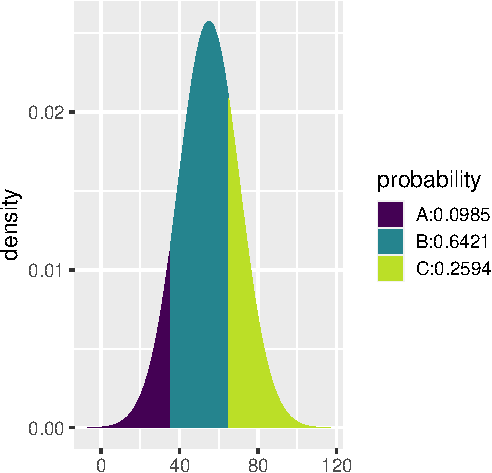
\includegraphics{004-pnorm-qnorm-exercise-solutions_files/figure-latex/unnamed-chunk-2-4} \end{center}

\begin{ShadedResult}
\begin{verbatim}
#  [1] 0.09846934 0.74058867
\end{verbatim}
\end{ShadedResult}

\begin{Shaded}
\begin{Highlighting}[]
\KeywordTok{pnorm}\NormalTok{(}\DataTypeTok{q =} \DecValTok{65}\NormalTok{, }\DataTypeTok{mean =} \DecValTok{55}\NormalTok{, }\DataTypeTok{sd =} \FloatTok{15.5}\NormalTok{) }\OperatorTok{-}\StringTok{ }\KeywordTok{pnorm}\NormalTok{(}\DataTypeTok{q =} \DecValTok{35}\NormalTok{, }\DataTypeTok{mean =} \DecValTok{55}\NormalTok{, }\DataTypeTok{sd =} \FloatTok{15.5}\NormalTok{)}
\end{Highlighting}
\end{Shaded}

\begin{ShadedResult}
\begin{verbatim}
#  [1] 0.6421193
\end{verbatim}
\end{ShadedResult}

\hypertarget{osteoporosis}{%
\section{Osteoporosis}\label{osteoporosis}}

Osteoporosis is a condition in which the bones become brittle due to
loss of minerals. To diagnose osteoporosis, an elaborate apparatus
measures bone mineral density (BMD). BMD is usually reported in
standardized form. The standardization is based on a population of
healthy young adults. The Wolrd Health Organization (WHO) criterion for
osteoporosis is a BMD 2.5 or more standard deviations below the mean for
young adults. BMD measurements in a population of people who are similar
in age and sex roughly follow a standard normal distribution.

\begin{enumerate}
\def\labelenumi{\alph{enumi}.}
\tightlist
\item
  What percent of healthy young adults have osteoporosis?
\item
  Woman aged 70 to 79 are, of course, not young adults. The mean BMD in
  this age is about -2 on the standard scale for young adults. Suppose
  that the standard deviation is the same for young adults. What percent
  of this older population has osteoporosis?
\item
  Likewise, osteopenia is low BMD, defined by the WHO as a BMD between 1
  and 2.5 standard deviations below the mean of young adults. What
  percent of healthy young adults have osteopenia?
\item
  The mean BMD among women aged 70 to 79 is about -2 on the standard
  scale for young adults. Suppose that the standard deviation is the
  same as for young adults. What percent of this older population has
  osteopenia?
\end{enumerate}

\begin{Shaded}
\begin{Highlighting}[]
\CommentTok{# a)}
\NormalTok{mosaic}\OperatorTok{::}\KeywordTok{xpnorm}\NormalTok{(}\DataTypeTok{q =} \FloatTok{-2.5}\NormalTok{)}
\end{Highlighting}
\end{Shaded}

\begin{ShadedResult}
\begin{verbatim}
#  
\end{verbatim}
\end{ShadedResult}
\begin{ShadedResult}
\begin{verbatim}
#  If X ~ N(0, 1), then
\end{verbatim}
\end{ShadedResult}
\begin{ShadedResult}
\begin{verbatim}
#   P(X <= -2.5) = P(Z <= -2.5) = 0.00621
\end{verbatim}
\end{ShadedResult}
\begin{ShadedResult}
\begin{verbatim}
#   P(X >  -2.5) = P(Z >  -2.5) = 0.9938
\end{verbatim}
\end{ShadedResult}
\begin{ShadedResult}
\begin{verbatim}
#  
\end{verbatim}
\end{ShadedResult}

\begin{center}
\includegraphics{004-pnorm-qnorm-exercise-solutions_files/figure-latex/unnamed-chunk-3-1} \end{center}

\begin{ShadedResult}
\begin{verbatim}
#  [1] 0.006209665
\end{verbatim}
\end{ShadedResult}

\begin{Shaded}
\begin{Highlighting}[]
\CommentTok{# b)}
\NormalTok{mosaic}\OperatorTok{::}\KeywordTok{xpnorm}\NormalTok{(}\DataTypeTok{q =} \FloatTok{-2.5}\NormalTok{, }\DataTypeTok{mean =} \DecValTok{-2}\NormalTok{, }\DataTypeTok{sd =} \DecValTok{1}\NormalTok{)}
\end{Highlighting}
\end{Shaded}

\begin{ShadedResult}
\begin{verbatim}
#  
\end{verbatim}
\end{ShadedResult}
\begin{ShadedResult}
\begin{verbatim}
#  If X ~ N(-2, 1), then
\end{verbatim}
\end{ShadedResult}
\begin{ShadedResult}
\begin{verbatim}
#   P(X <= -2.5) = P(Z <= -0.5) = 0.3085
\end{verbatim}
\end{ShadedResult}
\begin{ShadedResult}
\begin{verbatim}
#   P(X >  -2.5) = P(Z >  -0.5) = 0.6915
\end{verbatim}
\end{ShadedResult}
\begin{ShadedResult}
\begin{verbatim}
#  
\end{verbatim}
\end{ShadedResult}

\begin{center}
\includegraphics{004-pnorm-qnorm-exercise-solutions_files/figure-latex/unnamed-chunk-3-2} \end{center}

\begin{ShadedResult}
\begin{verbatim}
#  [1] 0.3085375
\end{verbatim}
\end{ShadedResult}

\begin{Shaded}
\begin{Highlighting}[]
\CommentTok{# c) }
\NormalTok{mosaic}\OperatorTok{::}\KeywordTok{xpnorm}\NormalTok{(}\DataTypeTok{q =} \KeywordTok{c}\NormalTok{(}\OperatorTok{-}\FloatTok{2.5}\NormalTok{,}\OperatorTok{-}\DecValTok{1}\NormalTok{))}
\end{Highlighting}
\end{Shaded}

\begin{ShadedResult}
\begin{verbatim}
#  
\end{verbatim}
\end{ShadedResult}
\begin{ShadedResult}
\begin{verbatim}
#  If X ~ N(0, 1), then
\end{verbatim}
\end{ShadedResult}
\begin{ShadedResult}
\begin{verbatim}
#   P(X <= -2.5) = P(Z <= -2.5) = 0.00621   P(X <= -1.0) = P(Z <= -1.0) = 0.15866
\end{verbatim}
\end{ShadedResult}
\begin{ShadedResult}
\begin{verbatim}
#   P(X >  -2.5) = P(Z >  -2.5) = 0.9938    P(X >  -1.0) = P(Z >  -1.0) = 0.8413
\end{verbatim}
\end{ShadedResult}
\begin{ShadedResult}
\begin{verbatim}
#  
\end{verbatim}
\end{ShadedResult}

\begin{center}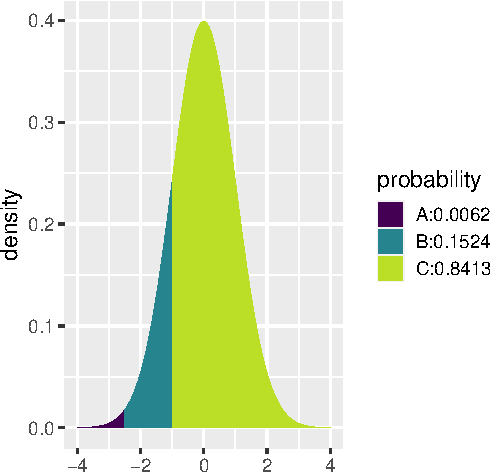
\includegraphics{004-pnorm-qnorm-exercise-solutions_files/figure-latex/unnamed-chunk-3-3} \end{center}

\begin{ShadedResult}
\begin{verbatim}
#  [1] 0.006209665 0.158655254
\end{verbatim}
\end{ShadedResult}

\begin{Shaded}
\begin{Highlighting}[]
\KeywordTok{pnorm}\NormalTok{(}\DataTypeTok{q =} \DecValTok{-1}\NormalTok{) }\OperatorTok{-}\StringTok{ }\KeywordTok{pnorm}\NormalTok{(}\DataTypeTok{q =} \FloatTok{-2.5}\NormalTok{)}
\end{Highlighting}
\end{Shaded}

\begin{ShadedResult}
\begin{verbatim}
#  [1] 0.1524456
\end{verbatim}
\end{ShadedResult}

\begin{Shaded}
\begin{Highlighting}[]
\CommentTok{# d)}
\KeywordTok{pnorm}\NormalTok{(}\DataTypeTok{q =} \DecValTok{-1}\NormalTok{, }\DataTypeTok{mean =} \DecValTok{-2}\NormalTok{) }\OperatorTok{-}\StringTok{ }\KeywordTok{pnorm}\NormalTok{(}\DataTypeTok{q =} \FloatTok{-2.5}\NormalTok{, }\DataTypeTok{mean =} \DecValTok{-2}\NormalTok{)}
\end{Highlighting}
\end{Shaded}

\begin{ShadedResult}
\begin{verbatim}
#  [1] 0.5328072
\end{verbatim}
\end{ShadedResult}

%\showmatmethods


\bibliography{pinp}
\bibliographystyle{jss}



\end{document}

